\section{Results}\label{sec:results} 

% The figures throughout the paper are
% best seen by zooming in to the electronic version of the paper.

% Figure: film reel of how a rerendered frame varies with change in head pose.

% 7.2) another main reason for would be due to our meticulous curating of the test set into multiple sub-test-sets characterized by the number of people in the shot, whether half or less than half of the person was captured in the frame, and how close the captured person(s) was to the camera.

The results for the experiments done on the baseline pretrained model and the variant retrained on only the video-chat-relevant Mannequin Challenge dataset are presented in this section. As of this writing generator\_test.py is only able to pick random pairs of reference and target frames from the 333 test-yes/ videos. The results for sequential pair picking, which would avoid possible repetition of picked pairs and allow for an exhaustive coverage of the test set, will replace the results below in a subsequent manuscript of this thesis shortly alongside the results for the variant trained on both the Mannequin Challenge and RealEstate10K datasets and more visually applealing/insightful graphs. Moreover, the number of training iterations/steps will be much more than the current 10k steps which is projected to increase the accuracy even more. 

An LPIPS value of 0 indicates there is either a perfect match between the images being compared or the images being compared are one and the same. To the contrary, SSIM values of 1 indicate a perfect match. Both these metrics range from 0 to 1. PSNR values, measured in decibels (dB), don't generally have an upper limit but values 20 dB or higher are considered acceptable. In calibrating our implementations of these metrics, when we compared an image with itself, we found the mean LPIPS, SSIM and PSNR values over 300 images to be  

% \begin{appendices}

\newcolumntype{L}{>{\raggedleft\arraybackslash}m{3.5cm}}
\newcolumntype{M}{>{\raggedright\arraybackslash}m{2cm}}
\newcolumntype{N}{>{\centering\arraybackslash}m{1.5cm}}
\newcolumntype{O}{>{\centering\arraybackslash}m{3cm}}

\begin{table*}[t]
% \begin{sidewaystable*}[t]
    \centering
    \begin{tabular}{ML|NN|NN}
    \toprule
    
    & & \multicolumn{2}{O}{\textbf{LPIPS $\downarrow$} target\_image vs rendered\_image} & \multicolumn{2}{O}{\textbf{LPIPS $\downarrow$} reference\_image vs target\_image} \\
    
    \cmidrule(lr){3-4} \cmidrule(lr){5-6}
    
    \textbf{Model Variant} & \textbf{Dataset(s) (re)trained on / No. of Videos} & n = 5 & n = 10 & n = 5 & n = 10 \\
    \midrule
    
    Pretrained & RealEstate10K / $\sim$70k & 0.418 & 0.525 & 0.446 & 0.555 \\
    
    \cmidrule(lr){1-2} \cmidrule(lr){3-4} \cmidrule(lr){5-6}
    
    Recreated & Mannequin Challenge / 1841 & 0.319 & 0.433 & 0.446 & 0.555 \\
    
    \cmidrule(lr){1-2} \cmidrule(lr){3-4} \cmidrule(lr){5-6}
    
    Recreated  & Mannequin Challenge + RealEstate10K & -- & -- & -- & -- \\
    
    \cmidrule(lr){1-2} \cmidrule(lr){3-4} \cmidrule(lr){5-6}
    
    Recreated multi-GPU & Mannequin Challenge & 0.418 & 0.525 & 0.446 & 0.555 \\
    
    \bottomrule
    \end{tabular}
    \caption{LPIPS Mean Values}
    \label{tab:lpips}
    {\small n refers to the distance between the reference and target frames picked by the generator. Retraining promises marked improvement over original pretrained model.}
\end{table*}
% \end{sidewaystable*}

\begin{table*}[t]
% \begin{sidewaystable*}[t]
    \centering
    \begin{tabular}{ML|NN|NN}
    \toprule
    
    & & \multicolumn{2}{O}{\textbf{SSIM $\uparrow$} target\_image vs rendered\_image} & \multicolumn{2}{O}{\textbf{SSIM $\uparrow$} reference\_image vs target\_image} \\
    
    \cmidrule(lr){3-4} \cmidrule(lr){5-6}
    
    \textbf{Model Variant} & \textbf{Dataset(s) (re)trained on / No. of Videos} & n = 5 & n = 10 & n = 5 & n = 10 \\
    \midrule
    
    Pretrained & RealEstate10K / $\sim$70k & 0.549 & 0.492 & 0.418 & 0.370 \\
    
    \cmidrule(lr){1-2} \cmidrule(lr){3-4} \cmidrule(lr){5-6}
    
    Recreated & Mannequin Challenge / 1841 & 0.560 & 0.494 & 0.418 & 0.370 \\
    
    \cmidrule(lr){1-2} \cmidrule(lr){3-4} \cmidrule(lr){5-6}
    
    Recreated  & Mannequin Challenge + RealEstate10K & -- & -- & -- & -- \\
    
    \cmidrule(lr){1-2} \cmidrule(lr){3-4} \cmidrule(lr){5-6}
    
    Recreated multi-GPU & Mannequin Challenge & 0.549 & 0.492 & 0.418 & 0.555 \\
    
    \bottomrule
    \end{tabular}
    \caption{SSIM Mean Values}
    \label{tab:ssim}
    {\small n refers to the distance between the reference and target frames picked by the generator. Retraining promises marked improvement over original pretrained model.}
\end{table*}
% \end{sidewaystable*}

\begin{table*}[t]
% \begin{sidewaystable*}[t]
    \centering
    \begin{tabular}{ML|NN|NN}
    \toprule
    
    & & \multicolumn{2}{O}{\textbf{PSNR $\uparrow$} target\_image vs rendered\_image} & \multicolumn{2}{O}{\textbf{PSNR $\uparrow$} reference\_image vs target\_image} \\
    
    \cmidrule(lr){3-4} \cmidrule(lr){5-6}
    
    \textbf{Model Variant} & \textbf{Dataset(s) (re)trained on / No. of Videos} & n = 5 & n = 10 & n = 5 & n = 10 \\
    \midrule
    
    Pretrained & RealEstate10K / $\sim$70k & 16.105 & 14.088 & 13.185 & 11.589 \\
    
    \cmidrule(lr){1-2} \cmidrule(lr){3-4} \cmidrule(lr){5-6}
    
    Recreated & Mannequin Challenge / 1841 & 16.729 & 14.664 & 13.185 & 11.589 \\
    
    \cmidrule(lr){1-2} \cmidrule(lr){3-4} \cmidrule(lr){5-6}
    
    Recreated  & Mannequin Challenge + RealEstate10K & -- & -- & -- & -- \\
    
    \cmidrule(lr){1-2} \cmidrule(lr){3-4} \cmidrule(lr){5-6}
    
    Recreated multi-GPU & Mannequin Challenge & 16.105 & 14.088 & 13.185 & 11.589 \\
    
    \bottomrule
    \end{tabular}
    \caption{PSNR Mean Values}
    \label{tab:psnr}
    {\small n refers to the distance between the reference and target frames picked by the generator. Retraining promises marked improvement over original pretrained model.}
\end{table*}
% \end{sidewaystable*}

% % \end{appendices}

These metrics mean value tables produced via the random reference, target pair experiments so far validate hypothesis A of this thesis by showing that transfer learning with completely unfrozen layers seems to be helping the 2020 Single-View MPI pick up from where it left off by specializing and improve upon its performance in accurately predicting close up shots of people in video-chat-relevant frames. 

A further testimony to this improvement can be obtained by inspecting the performance of even the prematurely halted multi-GPU variant. It performs at par with the original pretrained model which indicates that the pretained model has begun to continue where it left off and specialize in processing video-chat-like frames. It would have run properly if not for the resource errors mentioned in the previous section that could point to underlying issuess like possible unchecked growth of TensorFlow graphs per pipeline replica or something else. This seems to be the case even though the replicas seem to be getting properly allocated inputs and their respective outputs also seem to be getting well gelled together in the end.

The authors of 2020 MPI paper used the following pointers like the handling of occluded content, the production unpleasant artifacts at the edges of foreground objects, and so on to qualitatively compare the discrepancies in the results generated by each variant model. In addition to visually checking for these, we, like the authors also found that visually checking the disparity maps is also useful in verifying the quality of the MPI produced.   

\begin{figure}[!h]
\begin{tabular}{cccc}
\subfloat[reference]{\includegraphics[width = 1.3in]{figures/pretrained-5-apt/000000_image_reference.png}} &
\subfloat[target]{\includegraphics[width = 1.3in]{figures/pretrained-5-apt/000000_image_target.png}} &
\subfloat[disparity]{\includegraphics[width = 1.3in]{figures/pretrained-5-apt/000000_image_disparity.png}} &
\subfloat[rendered]{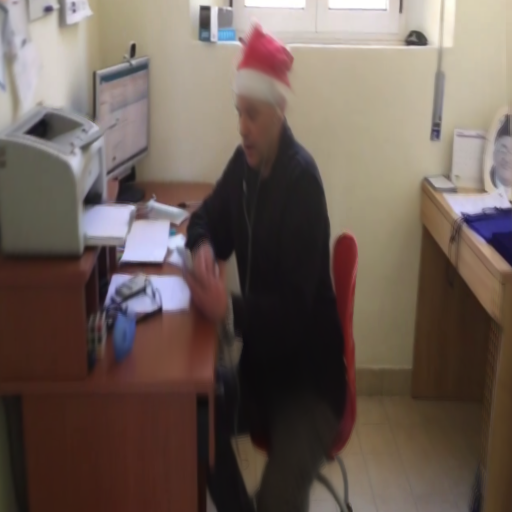
\includegraphics[width = 1.3in]{figures/pretrained-5-apt/000000_image_render.png}}\\
\subfloat[reference]{\includegraphics[width = 1.3in]{figures/mann-1841-5-apt/000000_image_reference.png}} &
\subfloat[target]{\includegraphics[width = 1.3in]{figures/mann-1841-5-apt/000000_image_target.png}} &
\subfloat[disparity]{\includegraphics[width = 1.3in]{figures/mann-1841-5-apt/000000_image_disparity.png}} &
\subfloat[rendered]{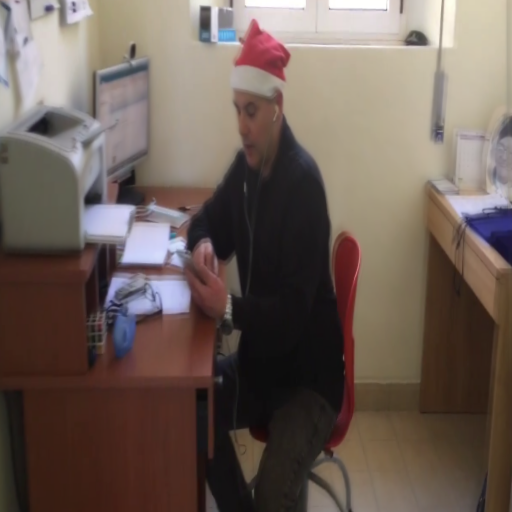
\includegraphics[width = 1.3in]{figures/mann-1841-5-apt/000000_image_render.png}}\\
\subfloat[reference]{\includegraphics[width = 1.3in]{figures/pretrained-10-apt/000000_image_reference.png}} &
\subfloat[target]{\includegraphics[width = 1.3in]{figures/pretrained-10-apt/000000_image_target.png}} &
\subfloat[disparity]{\includegraphics[width = 1.3in]{figures/pretrained-10-apt/000000_image_disparity.png}} &
\subfloat[rendered]{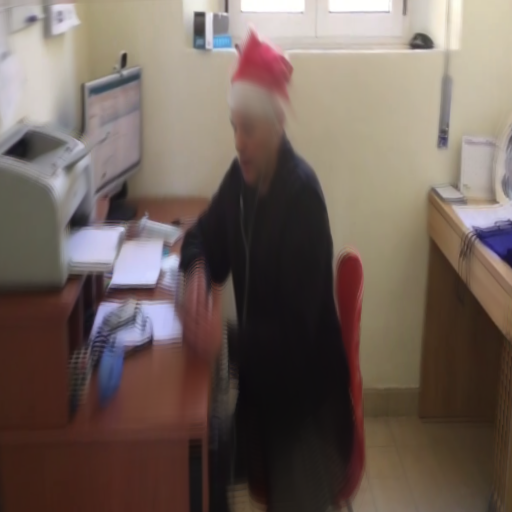
\includegraphics[width = 1.3in]{figures/pretrained-10-apt/000000_image_render.png}}\\
\subfloat[reference]{\includegraphics[width = 1.3in]{figures/mann-1841-10-apt/000000_image_reference.png}} &
\subfloat[target]{\includegraphics[width = 1.3in]{figures/mann-1841-10-apt/000000_image_target.png}} &
\subfloat[disparity]{\includegraphics[width = 1.3in]{figures/mann-1841-10-apt/000000_image_disparity.png}} &
\subfloat[rendered]{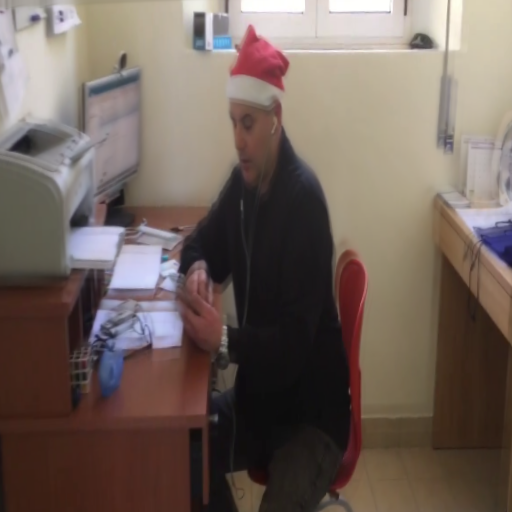
\includegraphics[width = 1.3in]{figures/mann-1841-10-apt/000000_image_render.png}}
\end{tabular}
\caption{Model Variants' Output Visualizations}
    {\small First Row: Pretrained Model -- tested 5 frames apart; Second Row: Retrained Model -- trained on 1841 Mannequin Challenge videos -- tested 5 frames apart; Third Row: Pretrained Model -- tested 10 frames apart; Fourth Row: Retrained Model -- trained on 1841 Mannequin Challenge videos -- tested 10 frames apart}
\end{figure}